\documentclass[a4paper,12pt]{article} % тип документа
\usepackage[margin=1in]{geometry} % Поля

%  Русский язык
\usepackage[warn]{mathtext}
\usepackage[T2A]{fontenc}			% кодировка
\usepackage[utf8]{inputenc}			% кодировка исходного текста
\usepackage[english,russian]{babel}	% локализация и переносы
% Математика
\usepackage{amsmath,amsfonts,amssymb,amsthm,mathtools} 
\usepackage{wasysym}
%%%
\usepackage{graphicx}

\usepackage{tabularx}

\usepackage{gensymb} % знак градуса
\usepackage{enumitem} % изменить список enumerate
\usepackage{placeins} % \FloatBarrier

\renewcommand{\thesection}{\Roman{section}} 
\renewcommand{\thesubsection}{\roman{subsection}}


\begin{document}

\newcolumntype{Y}{>{\centering\arraybackslash}X} %new tabularx


%титул
\hrule 	
\medskip
\begin{raggedright}
{\large \textbf{Отчёт по работе 4.4.3}}
\\
\medskip
{\Large Изучение призмы с помощью гониометра} 
\\
\medskip
{\large Карташов Констанин Б04-005}
\medskip
\hrule
\medskip
\end{raggedright}


\section{Анотация}

\paragraph{Цель работы:} 
Знакомство с работой и настройкой гониометра Г5, определение зависимости показателя преломления стекла призмы от длины волны, определение марки стекла и спектральных характеристик призмы.

\paragraph{Оборудование:}
\begin{itemize}
\renewcommand{\labelitemi}{$\triangleright$}
\itemsep0em
\item Гониометр
\item Ртутная лампа
\item Призма
\end{itemize}


\medskip\hrule\medskip

\section{Теоретическая часть}

\begin{figure}[h]
\center
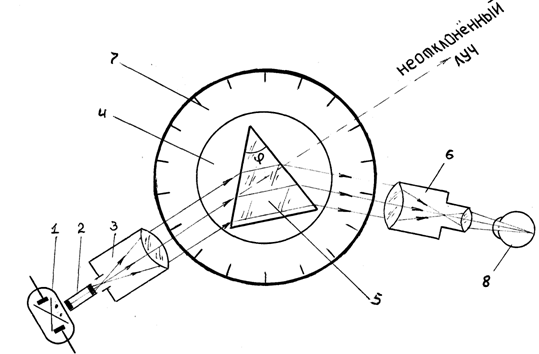
\includegraphics[width=0.7\textwidth]{gon.png}
\caption{Схема экспериментальной установки}
\label{fig:setup}
\end{figure}

\paragraph{Экспериментальная установка} состоит из гониометра, призмы и ртутной лампы. Схема установки представлена на рис. \ref{fig:setup}. Гониометр состоит из: коллиматора (3), в который поступает свет с ртутной лампы (1), подвижного столика (4), на котором размещена призма (5) так, чтобы через неё проходил свет из коллиматора, и объектива (6), собирающий преломлённые лучи. Угол между осью коллиматора и осью объектива измеряется по лимбу (7).

\paragraph{Спектр ртутной лампы} состоит из нескольких полос. Мы проводим измерения на самых ярких из них (рис. \ref{fig:spectrum} и табл. \ref{t:spectrum}).


\begin{figure}
\center
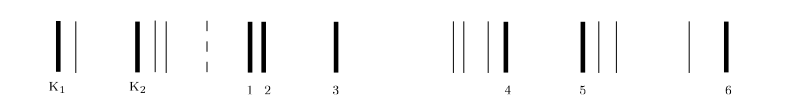
\includegraphics[width=\textwidth]{spectrum.png}
\caption{Спектр ртутной лампы}
\label{fig:spectrum}
\end{figure}

\begin{table}
\center
\begin{tabularx}{\textwidth}{|Y|Y|Y|Y|Y|Y|Y|Y|Y|}
\hline
№ & K1 & K2 & 1 & 2 & 3 & 4 & 5 & 6 \\
\hline
$\lambda$, нм & 690.7 & 623.4 & 579.1 & 577.1 & 546.1 & 491.6 & 436.8 & 404.7 \\
\hline 
Цвет & красн. & красн. & желт. & желт. & зелен. & голуб. & синий & фиолет. \\
\hline
\end{tabularx}
\caption{Длины волн ярких линий спектра ртутной лампы}
\label{t:spectrum}
\end{table}

\begin{figure}[h]
\center
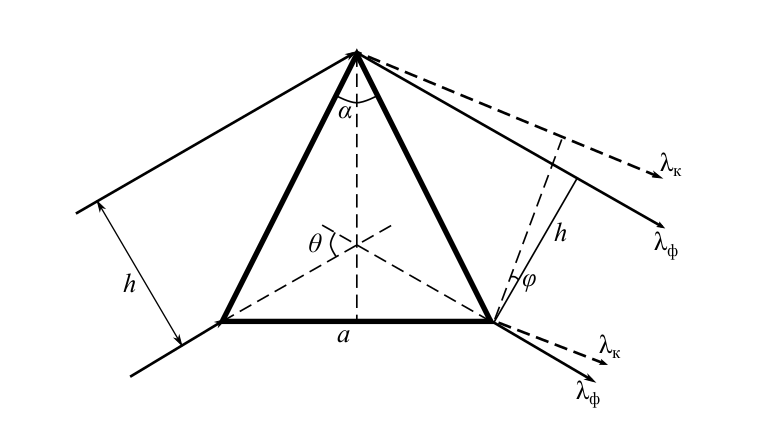
\includegraphics[width=0.7\textwidth]{prism.png}
\caption{Прохождения луча через призму}
\end{figure}


\paragraph{Дисперсия света в призме} При прохождении через призму лучи света с разными длинами волн преломляются в разной степени. Наименьший угол преломления получается, когда луч света идёт параллельно основанию призмы. В этом случае коэффициент преломления для луча можно рассчитать по формуле:

\begin{equation}
n(\lambda) = \frac{\sin \frac{\alpha + \varphi (\lambda)}{2}}{sin \frac{\alpha}{2}}.
\label{e:n}
\end{equation}

\paragraph{Угловая дисперсия} характеризует угловое расстояние между близкими спектральными линиями:

\[
D(\lambda) = \frac{d\varphi}{d\lambda},
\]

\noindent для призмы выполняется равенство:

\begin{equation}
D = \frac{d\varphi}{d\lambda} = \frac{a}{h} \frac{dn}{d\lambda}.
\label{e:disp}
\end{equation}



\medskip\hrule\medskip

\section{Экспериментальная часть}

\paragraph{} Проведём юстировку гониометра и определим начало отсчёта. За начало отсчёта берётся значение гониометра, при котором оси окуляра и коллиматора совпадают, в этой работе было выставлено начало отсчёта $180 \degree 1'0''$, далее все значения углов будут указаны с учётом начала отсчёта.

\paragraph{} Установим на столик призму, и повторно выровняем столик. Затем найдём преломляющий угол призмы, для этого найдём углы, при которых в центре объектива виден крест отражённый от рабочих поверхностей призмы:

\[
\begin{array}{l}
\varphi_1 = 235 \degree 51 ' 11 '', \\
\varphi_2 = 118 \degree 49' 45 '' , \\
\Delta \varphi = 117 \degree 01' 26'', \\
\alpha = 180 \degree - \Delta \varphi = 62 \degree 58 ' 34 '', \\
\end{array}
\]

\noindent где $\Delta \varphi$ -- угол между перпендикулярами к рабочим поверхностям призмы, $alpha$ -- преломляющий угол призмы. Приборная погрешность измерений -- одна секунда. При переводе в радианы получаем:

\[
\alpha = 62 \degree 58 ' 34 '' \pm 1'' = 1.099140 \pm 0.000005 \; \text{рад}.
\]

\noindent Далее величину $\alpha$ будем считать без погрешности, так как её погрешность значительно меньше угловой ширины наблюдаемых спектральных линий ($\sim 30''$).

\paragraph{} Теперь повернём столик так, чтобы одна рабочая поверхность призмы была направлена к источнику света, с другой стороны призмы будет виден спектр. Для каждой спектральной линии найдём положение призмы, при котором угол между ей и осью коллиматора будет минимальным. Запишем угол наименьшего преломления для каждой из спектральных полос. Затем пользуясь формулой (\ref{e:n}) найдём показатель преломления соответствующий каждой из полос. Все данные приведены в таблице (\ref{t:angles}).

\begin{table}[h]
\center
\begin{tabularx}{0.7\textwidth}{|c|X|X|X|}
\hline
Линия & $\varphi$ & $\varphi$, рад & $n$ \\ \hline
1 &	$51 \degree 57 ' 24  ''$&	0.9068 &	1.6141 \\ \hline
2 &	$51 \degree 58 ' 49 '' $&	0.9072 &	1.6143 \\\hline
3 &	$52 \degree 18 ' 55 '' $&	0.9131 &	1.6173 \\\hline
4 &	$53 \degree 5 ' 45 ''  $&	0.9267 &	1.6243 \\\hline
5 &	$54 \degree 17 ' 41 '' $&	0.9476 &	1.6348 \\\hline
6 &	$55 \degree 15 ' 46 '' $&	0.9645 &	1.6431 \\\hline
K1 &	$51 \degree 6 ' 59 ''  $&	0.8921 &	1.6065 \\\hline
K2 &	$51 \degree 35 ' 1 ''  $&	0.9003 &	1.6107 \\\hline
\end{tabularx}
\caption{Углы наименьшего преломления и показатели преломления}
\label{t:angles}
\end{table}

В качестве погрешности угла $\varphi$ можно взять угловую полуширину ширину линии $\delta \varphi / 2 = 15''$. Другим фактором является то, что во время работы несколько раз был смещён коллиматор, после чего приходилось заново устанавливать начало отсчёта. При повторном измерении углов наименьшего преломления значения расходились в пределах $\Delta \varphi \approx 30''$ поэтому в качестве погрешности возьмём $\Delta \varphi = 30'' = 1.5 \cdot 10^{-4}$ рад.

Погрешность показателя преломления найдём из формулы (\ref{e:n}):

\[
dn(\lambda) = \frac{1}{2}\frac{\cos{\frac{\alpha + \varphi(\lambda)}{2}}}{\sin{\frac{\alpha}{2}}} d \varphi(\lambda) = \lbrace \varphi \approx 0.9, \; \alpha \approx 1.1 \rbrace = \frac{1}{2} \frac{\cos{\frac{1.1 + 0.9}{2}}}{\sin{\frac{1.1}{2}}} d \varphi(\lambda) \approx 0.5 d\varphi(\lambda),
\]

\noindent получим $\Delta n \approx 1 \cdot 10^{-4}$.

\paragraph{} По точками из таблицы \ref{t:angles} построим график зависимости показателя преломления от длины волны (рис. \ref{fig:plot}). Для полос 1-6 проведём наилучшею прямую методом наименьших квадратов, угол наклона будет $- (1.6 \pm 0.1) \cdot 10^{-4}$ нм$^{-1} = (1.6 \pm 1) \cdot 10^{3}$ см$^{-1}$.

\begin{figure}[h]
\center
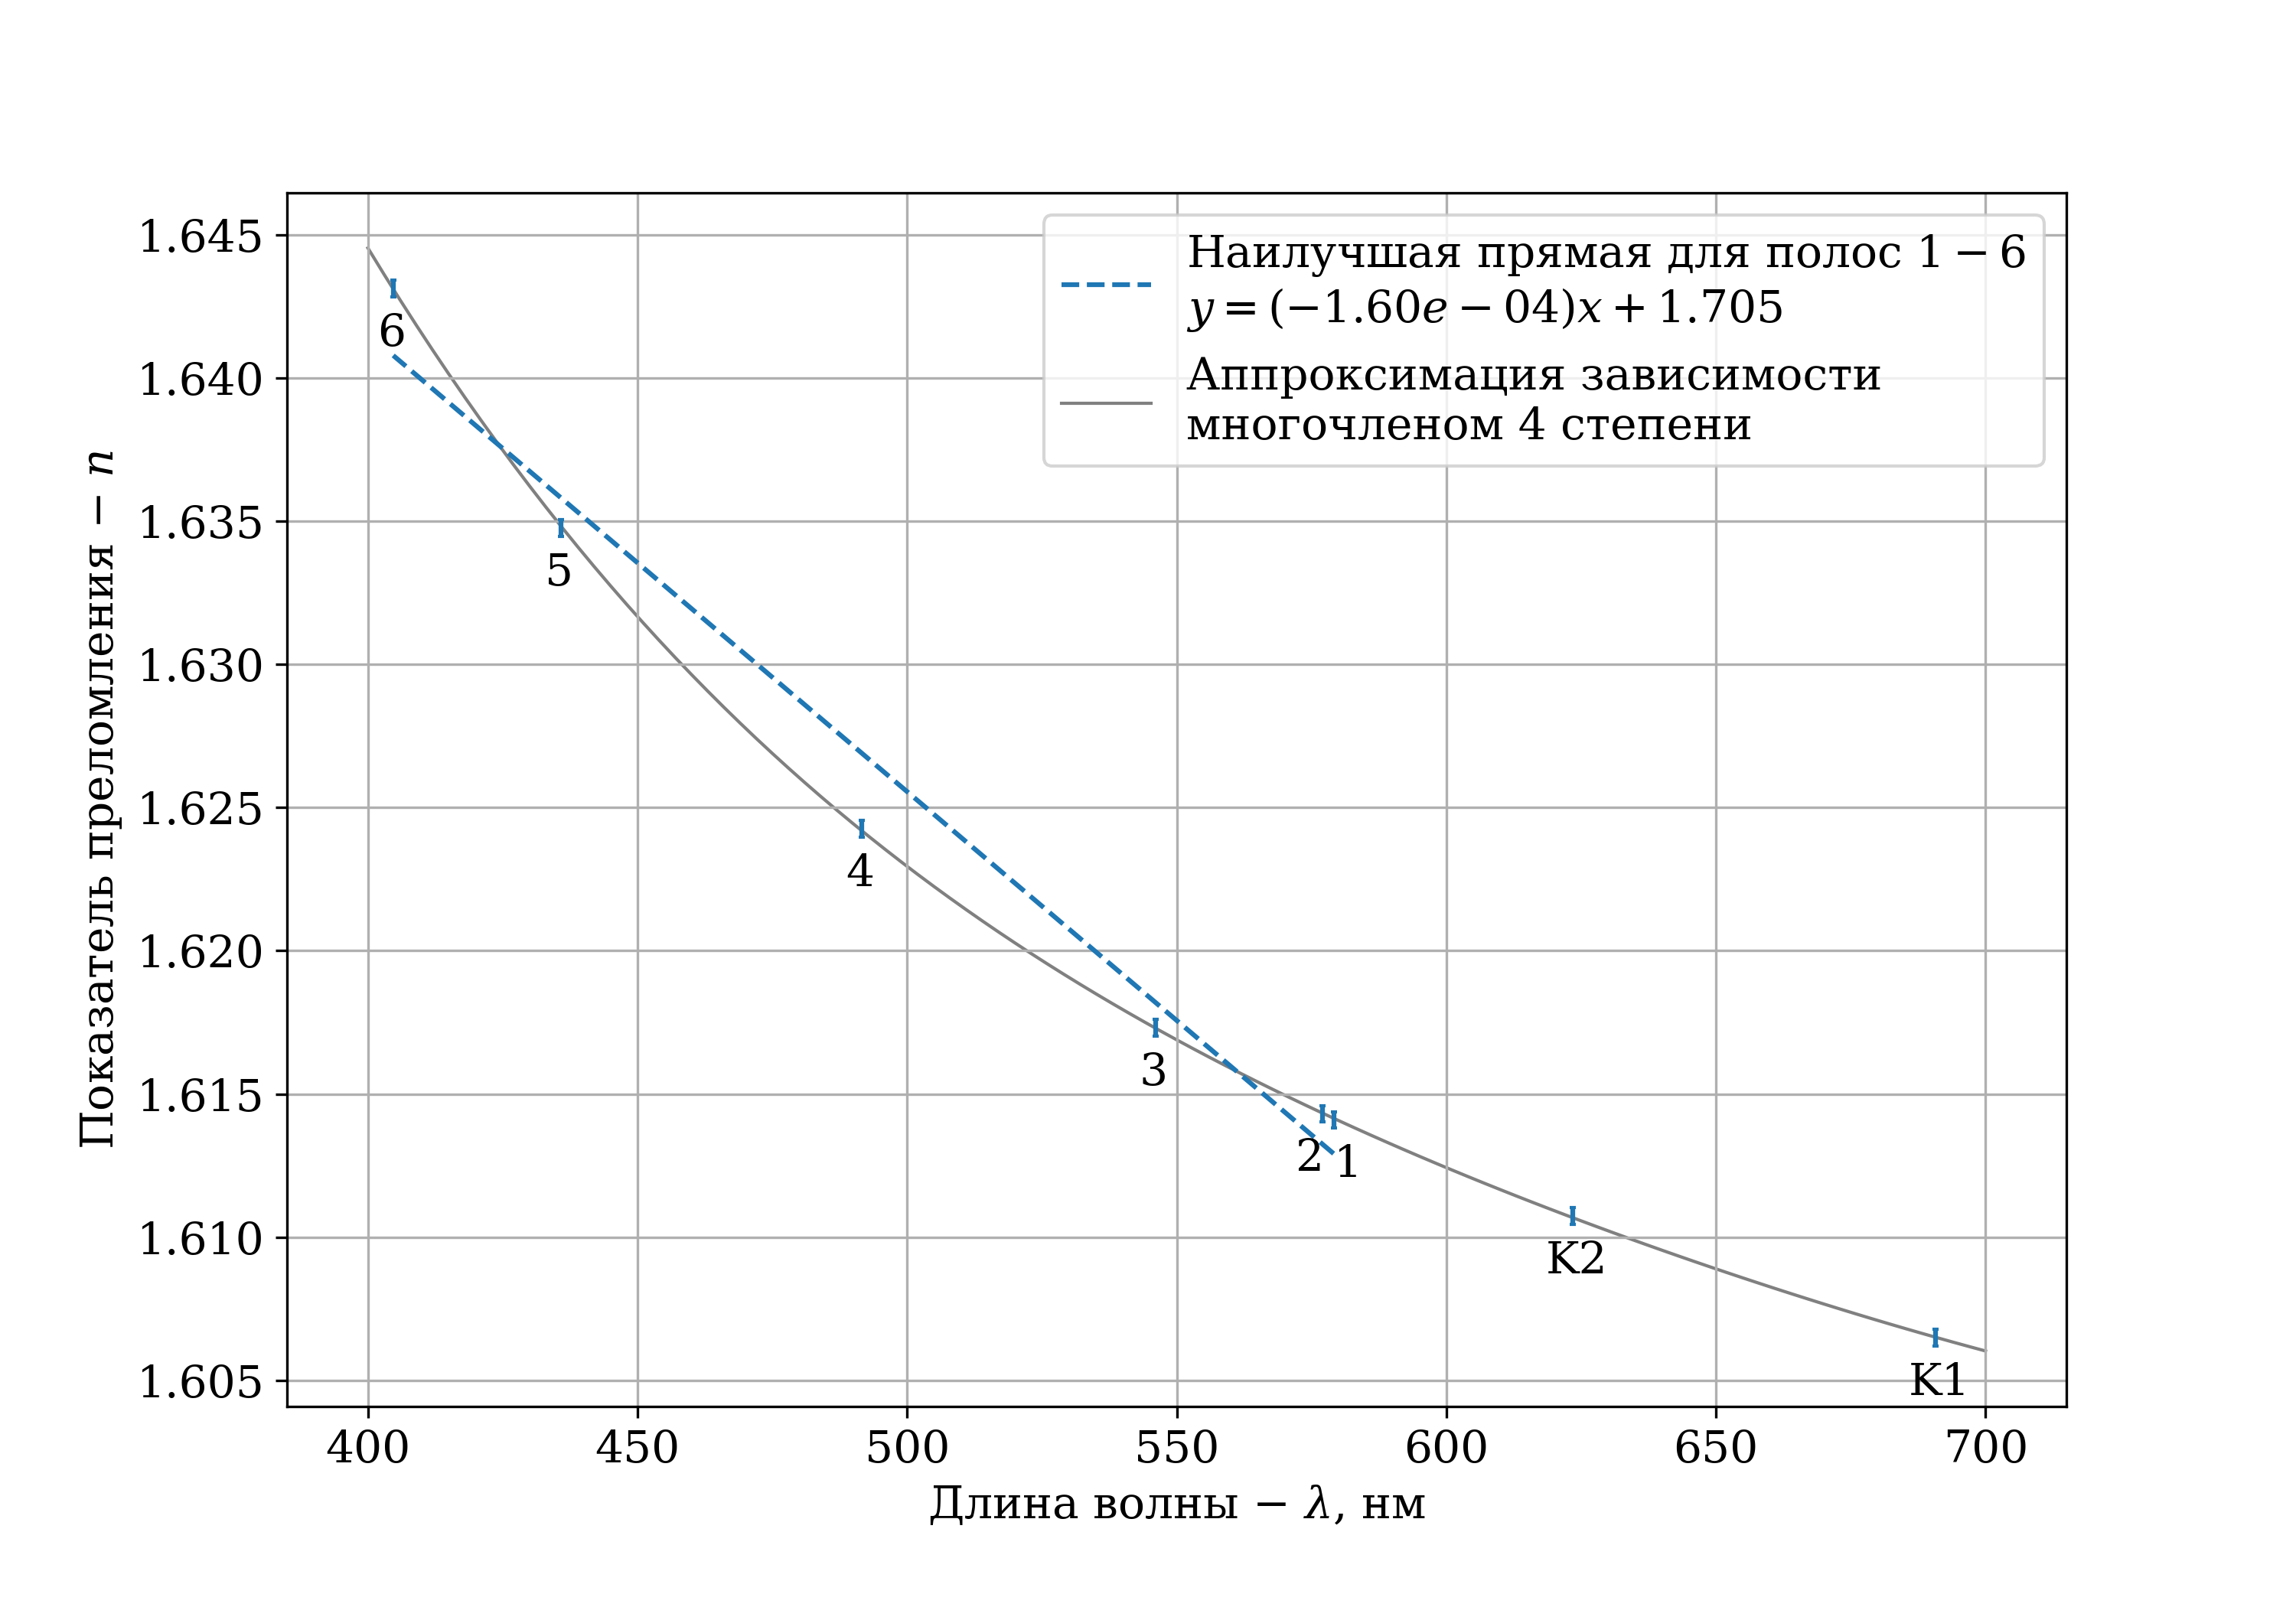
\includegraphics[width=\textwidth]{plot1.png}
\caption{Зависимость показателя преломления от длины волны}
\label{fig:plot}
\end{figure}

\paragraph{} Угловое расстояние между линиями жёлтого дублета $\Delta \varphi = 2'10''$, а разность длин волны $\Delta \lambda = 2.1$ нм. По формуле (\ref{e:disp}) получим:

\[
\frac{\Delta \varphi}{\Delta \lambda} = \frac{a}{h} \frac{dn}{d\lambda} \; \Rightarrow \; \frac{a}{h} = \frac{\Delta \varphi}{\Delta n} = \frac{6.3 \cdot 10^{-4}}{2 \cdot 10^{-4}} \approx 3.
\]

\paragraph{} При геометрическом расчёте, считая угол преломления $\alpha = 60 \degree$ и коэффициент преломления $n = 1.614$ получаем $a/h \approx 1.47$. 

\paragraph{} Угловая дисперсия по формуле (\ref{e:disp}): $D = 3.1 \cdot 10^{-4}$ нм$^{-1}$. Максимально разрешимий спектральный интервал $\delta \lambda = \delta \varphi / D$, где $\delta \varphi$ -- угловая полуширина спектральной линии, получаем $\delta \lambda = 15'' / (3.1 \cdot 10^{-4}) \approx 0.24$ нм. 

\paragraph{} Разрешающая способность оптического прибора $R = \frac{\lambda}{\delta \lambda} \approx \frac{580}{0.24} = 2400$.

\paragraph{} Максимальная разрешающая способность призмы: $R = a \left| \frac{dn}{d\lambda} \right| = 7.2 \cdot 1.6 \cdot 10^{3} \approx 11500$.

\medskip\hrule\medskip

\section{Выводы}

\begin{enumerate}
\item В ходе работы	 качественно пронаблюдали эффект дисперсии в призме.
\item Нашли зависимость коэффициента преломления от длины волны. Получили зависимость похожею на теоретическую. 
\item По наклону кривой оценили среднею дисперсию стекла. Получили $\frac{dn}{d\lambda} \approx -1.6 \cdot 10^{3}$ см$^{-1}$, что может лежать в пределах значения для стекла TФ-1
\item Рассчитав угловую дисперсию по наблюдаемой картинке $D = 7.9 \cdot 10^2 $ см$^{-1}$, нашли разрешающую способность $R \approx 2400$, что меньше теоретической максимальной разрешающей способности в 4 раза. Из этого можно сделать вывод, что в дифракции была задействована лишь малая часть призмы.
\end{enumerate}



\medskip\hrule\medskip

\end{document}
